\chapter{Approaches}

\begin{figure}[hbt]
	\centering
	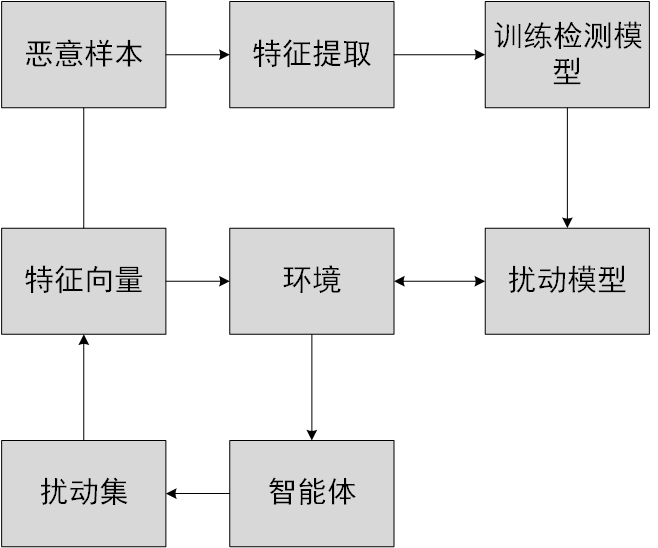
\includegraphics[width=0.75\textwidth]{figures/3.1}
	% \caption[这里的文字将会显示在 listoffigure 中]{这里的文字将会显示在正文中}
	\caption{Common Adversarial Malware Generation Model Structure}\label{fig:3.1}
\end{figure}


\section{Approaches Conclusion}
To address current adversarial malware generation methods' limitations in coarse perturbation techniques, weak semantic control, lack of structural disturbance sequences, and neglect of practical costs and deployability, this research proposes an innovative adversarial sample generation framework. Common existing methods rely on simple, random byte insertions or section name modifications that lack effective control over sample legitimacy, semantic consistency, and executability, resulting in unstable evasion in real environments. Therefore, this research aims to solve these shortcomings by systematically optimizing multiple key aspects of adversarial sample generation.

Firstly, in the disturbance space modeling aspect, this paper introduces multidimensional disturbance techniques and breaks the limitation of traditional methods that solely rely on single disturbance methods. Since malware exhibits diverse features in different execution stages, this research designs a structural disturbance strategy with semantic awareness capacities, avoiding file functionality disruption and enhancing evasion difficulties. Secondly, targeting the disturbance legitimacy issue, a disturbance legitimacy control method based on semantic consistency is proposed to ensure adversarial samples evade detection while maintaining original functionality and behavioral consistency, avoiding instability from blind disturbances.

Furthermore, recognizing the obvious temporal dependency in disturbance sequences, this research employs the PPO algorithm combined with LSTM networks to model disturbance sequences, effectively capturing dynamic relationships between disturbances. This approach enhances the overall coherence, stealth, and deceptive nature of disturbance sequences, optimizing the order and strategies to further improve evasion capabilities.

Lastly, addressing the neglect of disturbance costs and executability, a new reward mechanism is proposed in this research. Except for focusing on evasion rates, it considers different factors such as resource consumption and execution time, ensuring that adversarial samples are not only highly aggressive but also deployable in real environments. This prevents sample size surges, prolonged runtime, or functional loss caused by excessive disturbances.

\section{Data Collection and Preprocessing}

High-quality data is fundamental to the adversarial sample generation system effective operation, especially dominant for ELF-format executable file research due to the current lack of authoritative, standardized public datasets. To bridge this gap, this research constructs a full-coverage, structurally diverse ELF sample set, including both malicious and benign samples, ensuring a robust experimental foundation and promotion capability for model training and disturbance strategy evaluation.

For malicious sample collection in this research, verified ELF-format malware samples targeting x86 architecture were sifted and downloaded from renowned open-source platforms such as VirusShare\cite{VirusShare} and Maltrieve. These samples cover common attack types, such as worm propagation programs, cryptocurrency miners, remote-controlled backdoors, DDoS tools, and embedded Trojans, offering strong representativeness and research value. To enhance sample quality, format validation, duplicate hash removal, and malicious behavior label verification were performed to ensure authenticity and consistency.For benign sample collection in this research, multiple target runtime environments were established using QEMU virtualization technology, including ARM-based embedded systems like Raspbian and OpenWrt, and x86-based systems like Ubuntu. Legitimate ELF programs, such as system tools, daemons, and configuration scripts were extracted from those embedded systems. These samples, being functionally complete and structurally standard, cover various development tool chains and build methods, enhancing the diversity and representativeness of the benign sample set.

To ensure dataset quality and accuracy, after initial sample collection, a review mechanism from the VirusTotal\cite{VirusTotal} platform was introduced for all collected ELF executable samples, strengthening the authority of label notes annotation and the credibility of maliciousness confirmation. In detail, first, hash fingerprints like SHA-256 are extracted from each sample to create unique identifiers, removing duplicate and redundant samples. Second, samples are uploaded to VirusTotal for comprehensive detection by using integrated multiple engines that contain Kaspersky, Avast, BitDefender, and ESET. 

In the scanning process, this research concentrates on critical information, including detection tags, malicious scores, behavioral analysis results and YARA rule matches returned by engines, which are used to construct a metadata report for each sample for subsequent analysis, training and evaluation. Besides, manual review and multi-round voting are introduced to judge and classify marginal samples that exhibit annotation inconsistency or significant engine disagreements, ensuring data annotation consistency and accuracy. Furthermore, information extracted from the scan reports, such as API call signatures, connection behaviors, and timestamps, also serves as a reference for subsequent disturbance design and adversarial sample generation, helping to identify key features prioritized by current detection mechanisms and guiding disturbance strategy selection.


\section{Disturbance Strategy Construction}

To counter modern malware detection systems' integrated analysis across static, dynamic, and behavioral features, this research proposes a hierarchical combined disturbance strategy that targets to disrupt traditional feature extraction chains through three levels—structural information, instruction sequences, and dynamic behaviors, enhancing the concealment and robustness of adversarial samples. Since current detection systems typically rely on fixed rules or trained models to extract static features, such as section structures, function call graphs, symbol info, instruction-level features, such as n-grams and CFG paths, and dynamic behaviors such as system call sequences, memory behaviors, thus, designing disturbance mechanisms effective against these detection paths is crucial for generating high-quality adversarial samples.

In structural disturbance aspect, this research mainly adopts structural transformation strategies based on insertion that exhibit high adaptivity and are not disruptive to original program functionalities. Concrete methods include inserting fake sections and invalid segments in ELF binary files, such as dynamically create sections that are only used for obfuscation and do not engage program logic processes, such as .fake and .dummy\_code, by using LIEF \cite{LIEF2025} library. Additionally, slight ELF Header, Program Header Table and Section Header Table adjustments, including altering section table sequences, fabricating the entry point address and adding relocation information, induce parsing errors in static analysis tools. Furthermore, packing and unpacking structural disturbance operations via compression tools like UPX, along with strategies to restore execution capability, confuse detection systems based on byte signature and structural pattern comparison. 

\begin{figure}[hbt]
	\centering
	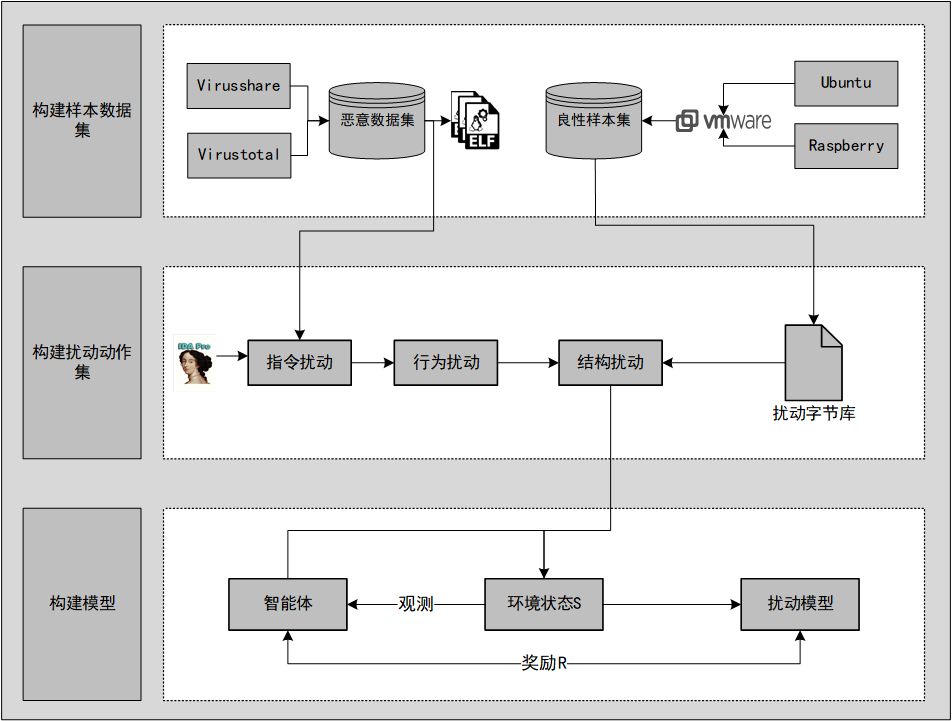
\includegraphics[width=0.75\textwidth]{figures/3.2}
	% \caption[这里的文字将会显示在 listoffigure 中]{这里的文字将会显示在正文中}
	\caption{Adversarial Sample Generation Framework Based On RL}\label{fig:3.2}
\end{figure}

In the instruction layer, this research used disassembly tools, such as IDA Pro and radare2, to disassemble original binary samples and extract control flow graphs to achieve instruction disturbance. First, in the background that program semantics are not disrupted, equivalent instruction replacements, such as using “xor eax, eax” to replace “mov eax, 0” and using redundant arithmetic chains to achieve simple assignments, disturb common semantic understanding for detection models. Second, utilizing register swapping strategies like replacing “eax” with “ebx” changes register usage patterns and modifies instruction jump logic. Indirect jumps and invalid jumps are introduced to increase CFG complexity to disturb static diagram analyzer targeted on CFG features with the premise that jump target is not changed. In the instruction combination realm, this research introduces invalid padding operations, such as NOP sled and empty function call sequences, to increase the difficulty of extracting meaningful semantic segments.

To address dynamic analysis system behavioral model features, this research design a dynamic execution disturbance mechanism aims to evade behavioral detection models based on sandbox techniques. This mechanism modifies the actual Entry Point, prioritizes executing fabricated behavioral logic and then gradually executes true malicious code, effectively postponing the exposure of factual behaviors in windows that capture behaviors. Common strategies include self-loop logic, such as fabricated loop structures, empty jump paths that do not affect program execution logic but prolong execution time and delayed APIs insertions, such as sleep() and nanosleep(), which prevent sandbox extraction workflows. Furthermore, virtual environment detection functions, such as CPUID instructions and MAC address identification instructions, can also be embedded to make samples exhibit different behaviors on platform based on virtual analysis. Combined with inserting invalid control flows into dynamic segments, these disturbance strategies demonstrate strong evasion capabilities during dynamic behavior analysis based on sandboxes.

\subsection{Structural Disturbance Methods}

In the adversarial malware sample generation process, structural level disturbances refer to introducing changes by modifying a file's internal structure. These changes commonly do not affect the file's execution logic but effectively evade traditional detection methods. Structural level disturbances include operations on sections, imported symbols, dynamic libraries, compression, and decompression, but are not limited to these.

These disturbances primarily concentrate on achieving the following purposes by altering certain elements in the file structure:

\begin{enumerate}
	 
\item Increasing file unpredictability: By randomizing or changing parts of the file, detection systems hardly identify the file, relying on fixed patterns.

\item Evading static analysis: Static analysis tools often depend on fixed file structural features, such as sections, symbol tables, and import tables. Disturbing these structures increases detection difficulty.

\item Avoiding signature matching: Some malware detection tools rely on known signatures, such as values, section structures from malicious samples. Disturbing structures creates differences between the file and the original malicious sample in these signatures, enabling evasion.
\end{enumerate}

(1)Section Disturbance

In ELF files, sections are the fundamental units, storing different types of data, such as code, data, symbols. Disturbing section content can modify file behavior or increase its complexity. Common section perturbation methods include:
\begin{enumerate}

\item Modifying section content: For example, appending random data to existing sections or replacing data in specific sections with benign data like harmless strings or binary content increases malicious files’ complexity and avoids matching known malicious sample signatures.

\item Renaming sections: Changing section names to common or random names makes it harder for detection tools to identify critical sections, especially the .text section that contains program code.

\end{enumerate}

The section disturbance design in this paper is listed in Table \ref{tab:4.1}.

\begin{table}[htbp]
	\centering
	\caption{Section Disturbance Type}\label{tab:4.1}
	\begin{tabular*}{\textwidth}{@{\extracolsep{\fill}}ccc}
		\toprule
		Disturbance Methods & Abbreviation & Effects \\
		\midrule
		section\_append & SA & appending random data to a randomly selected section (may alter the content and entropy of sections) \\
		add\_section\_benign\_data & ASBD & extracting an entire section from a benign file and add it to the target ELF \\
		add\_section\_strings & ASS & generating a new section filled with benign string content \\
		section\_rename & SR & randomly renaming a section using a name from common section names \\
		\bottomrule
	\end{tabular*}
\end{table}


(2) Imported Symbol and Library Disturbance

The dynamic symbol table in ELF files contains external functions or libraries that require runtime linking. Disturbing these symbols can make malware behavior more unpredictable. For example:
\begin{enumerate}
	
\item Adding malicious symbols: Inserting malicious dynamic symbols such as malicious function names into the file or mixing symbols with benign files to increase complexity.

\item Modifying library dependencies: Altering ELF dependency libraries that do not exist or are not common disrupts traditional static analysis processes.
\end{enumerate}
The imported symbol and library disturbances designed in this paper are listed in Table \ref{tab:4.2}.

\begin{table}[htbp]
	\centering
	\caption{Import Symbols and Library Disturbance}\label{tab:4.2}
	\begin{tabular*}{\textwidth}{@{\extracolsep{\fill}}ccc}
		\toprule
		Disturbance Methods & Abbreviation & Effects \\
		\midrule
		add\_imports & AI & 从 benign ELF 文件中添加一个动态符号到目标 ELF 中(如函数导入) \\
		add\_library & AL & 从 benign ELF 文件中添加一个共享库和其导入函数 \\
		\bottomrule
	\end{tabular*}
\end{table}



(3) Random Data Appending (Overlay)

Overlay techniques involve appending random data that is commonly harmless or disguised to the end of a file, altering its size and structure without changing execution logic. This technique is commonly used in malware to evade detection based on signature comparison. Common methods include:
\begin{enumerate}

\item Appending random bytes: Adding random byte sequences to the end of ELF files. This operation does not affect execution logic but may change file hashes, making the file evade traditional detection based on hash comparison.

\item Appending benign binary content: Inserting sections or binary content extracted from known benign files into malicious file increases complexity and disrupts static analysis tool detection.
\end{enumerate}

\begin{table}[htbp]
	\centering
	\caption{随机数据附加类型}\label{tab:4.3}
	\begin{tabular*}{\textwidth}{@{\extracolsep{\fill}}ccc}
		\toprule
		扰动方法 & 简写 & 效果 \\
		\midrule
		overlay\_append & OA & 在二进制文件的末尾附加随机内容 \\
		append\_benign\_data\_overlay & ABDO & 追加来自 benign ELF 文件 .text 段的内容 \\
		append\_benign\_binary\_overlay & ABBO & 直接追加整个 benign ELF 文件内容 \\
		add\_strings\_to\_overlay & ASTO & 追加来自 benign 字符串文件的内容(UTF-8 编码) \\
		\bottomrule
	\end{tabular*}
\end{table}

(4) Compression and Decompression (UPX Packing and Unpacking)

Compressing malicious files is another common disturbance technique. Compressing ELF files using tools like UPX can hide the original file structure and make the file non-executable without decompression. This approach primarily has the following features:
\begin{enumerate}

\item Compression: Compressed files alter the file's internal structure, making it appear entirely different from the original, thereby evading detection based on features.

\item Decompression: Compressed ELF files are decompressed to their original state during runtime, requiring an additional decompression step. This method allows malicious software behaviors and file structures to be hidden behind the compression layer, increasing the difficulty of reverse engineering and static analysis.
\end{enumerate}
\begin{table}[htbp]
	\centering
	\caption{压缩加壳类型}\label{tab:4.4}
	\begin{tabular*}{0.9\textwidth}{@{\extracolsep{\fill}}ccc}
		\toprule
		扰动方法 & 简写 & 效果 \\
		\midrule
		upx\_pack & UP & 使用 upx 对 ELF 文件进行压缩 \\
		upx\_unpack & UUP & 使用 upx -d 解压已压缩的 ELF 文件 \\
		\bottomrule
	\end{tabular*}
\end{table}

(5) go-bindata Toolbox in Go for Packaging ELF Files

go-bindata is a Go tool designed to convert binary files, such as ELF files, images, and audio files, into byte arrays within Go source code. In the malware analysis realm, embedding ELF files into Go programs effectively conceals their actual content and increases the difficulty of static analysis and reverse engineering. Specifically, the go\_bindata\_wrapper method converts ELF files into Go code to hide their functionalities in Go programs, which enables malicious files to evade common static detection and signature-matching tools.

First, convert the ELF file into Go source code using the go-bindata tool, generating a Go file containing the ELF file's byte data. Then, compile this Go code that contains the ELF byte data into a final Go executable program using the Go compiler. At runtime, the ELF file is read and recovered to execute its original operations.

(6) Section Header Table Modification

The target of section header table disturbances is altering the apparent characteristics of binary files by modifying specific metadata or header information, thereby disrupting detection tools or reverse analysis processes. This technique is commonly used in adversarial sample generation for malware analysis, aiming to help malicious programs evade traditional antivirus software or sandbox detection systems and increase analysis difficulty. Figure \ref{tab:4.5} introduces two section header table disturbance methods adopted in this paper.

\begin{table}[htbp]
	\centering
	\caption{节头表扰动类型}\label{tab:4.5}
	\begin{tabular*}{0.9\textwidth}{@{\extracolsep{\fill}}ccc}
		\toprule
		扰动方法 & 简写 & 效果 \\
		\midrule
		Remove Debug & RD & 在二进制文件中删除调试信息(用零填充) \\
		Break Checksum & BC & 在可选标题中删除校验和值(用零填充) \\
		\bottomrule
	\end{tabular*}
\end{table}



\subsection{Instruction Disturbance Methods}

In this research, powerful disassembly tools like IDA Pro are adopted to perform static analysis and code extraction on ELF-format malware samples, establishing a foundation for subsequent disturbance operations that ensure semantics. Although achieving fully precise disassembly remains challenging for stripped symbols like missing symbol tables and debugging information ELF executables on x86 architecture, advanced current disassemblers like IDA Pro can achieve high coverage for code generated from prevalent compilers through combined disassembly algorithms, recognition of specific code structures, and basic data-flow analysis. When processing ELF files, IDA Pro identifies symbol information and sections in the Program Header Table, such as .text, .plt, .rela, and .plt, enabling locating function boundaries accurately, recognizing control flow, and generating basic block graphs and function call graphs. This facilitates the extraction of semantically stable instruction regions for transformation.

\begin{figure}[hbt]
	\centering
	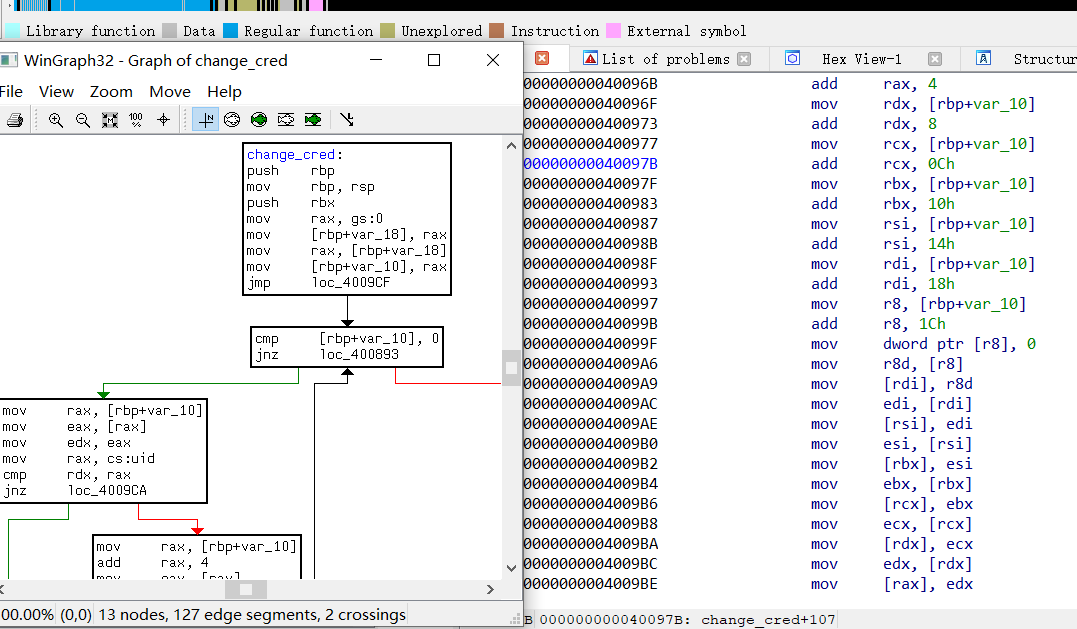
\includegraphics[width=0.75\textwidth]{figures/4.1}
	% \caption[这里的文字将会显示在 listoffigure 中]{这里的文字将会显示在正文中}
	\caption{IDA Disassembly CFG diagram}\label{fig:4.1}
\end{figure}


To ensure disturbances do not disrupt the original program logic, the disassembled instructions are first transformed into a custom Intermediate Representation (IR). This IR records each instruction's static semantic information, such as opcode, explicit and implicit operands, register read and write relationships, and impacted flag bits, which effectively aids in analyzing control and data dependencies to identify safely modifiable instruction regions. Subsequently, three disturbance techniques—Instruction Substitution, Instruction Reordering, and Register Reallocation—ensure semantics are implemented. These methods respectively introduce disturbances at the instruction level, sequential layer, and register usage level, aiming to enhance sample diversity and model robustness while preserving semantics.

During transformation, all modifications are limited to identified basic blocks free of control dependency conflicts, ensuring Program Control Flow Graph (CFG) stability. If transformations like instruction resequencing cause code address shifts, relevant relocation information, such as .rela section and .text section, in the ELF file is synchronously updated to prevent faulty function call and jump address. This process executes per ELF file independently, automatically generating multiple syntactically distinct yet semantically equivalent adversarial samples. These enhance diversity in training and testing phases, effectively improving the robustness of malware detection systems based on static analysis.

(1) Instruction Substitution

Instruction substitution serves as a binary code disturbance method that alters program structure by replacing original instructions with equivalent ones while preserving program functionality. It not only disrupts code appearance but also increases the difficulty for static analysis and reverse engineering. Details are described as follows:
\begin{enumerate}

\item Equivalent Instruction Replacement:

On x86 architecture, many instructions have multiple equivalent forms, same functionality can be achieved by different operands and instruction forms.For example, “add r/m32, r32” can be replaced with “add r32, r/m32”, these two instructions are equivalent while operands are registers.

For logic operations, “test r/m8, r8” is equivalent to “test r/m8, r/m8”.

Some arithmetic instructions also have multiple equivalent forms, such as “sub r/m32, r32” can be replaced with “neg r/m32”.

Operand forms can be altered when instructions are replaced, and do not affect ultimate calculation result. For example, “mov r32, r/m32” and “mov r/m32, r32” are equivalent operations, but the instruction byte expression can be altered by changing the sequence of source and target operands.

In some circumstances, replacing original instructions with instructions that are the same length but different in operations are permitted.
For example, “inc r32” can be replaced with “add r32, 1”, these two instructions have same functionality, different instruction length and coding.

“dec r32” can be replaced with “sub r32, 1”, these two instructions have same effect, but increase code's complexity.

\item Control Flow Instruction Replacement:

Control flow instructions, such as jump, conditional jump, and call, can be replaced with equivalent instructions. For example, “jmp label” can be replaced with “call label; pop”, although two instructions achieve same jump result, but their operands and instruction forms are different.

“je” can be replaced with “jne” by adjusting the flags properly to maintain functional consistency.

\item Maintain instruction length consistency:

Increasing instruction length may cause code structure to be broken in many stripped binary files; thus, it is vital to ensure that each replaced instruction's length should be the same as the original. This can be achieved by selecting equivalent instructions that have the same length, avoiding disrupting the program's overall layout.

\item The application method of randomized replacement:

Replacements can be applied according to certain rules or randomized equivalent instruction selection. Replacements may not be applied to each instruction but are selectively applied to specific code blocks relying on program characteristics and analysis results. This method can ensure that replacements do not affect the program's control flow and logic structure but alter the program's appearance, increasing static analysis difficulty.

\end{enumerate}

Through the methods above, instruction replacements not only maintain the program's complete functionalities but also increase the program's obfuscation, making it harder for static analysis tools to recognize the program's real intention and increasing the complexity of reverse engineering.

(2) Instruction Reordering
\begin{enumerate}


\item Intra Basic Block Reordering:

In a basic block, instructions without data and control dependencies can be reordered without affecting functionality. Since basic blocks are intermediate code areas for linear execution, and the compiler only selects one of equivalent sequences during machine code generation, thus instruction sequence modification does not affect the program's functionality if the dependency relationship remains unchanged.

This research disassembles target binaries to extract all basic blocks, then perform dependency analysis on each block, identifying each instruction's use and def register sets, constructing a Directed Acyclic Graph (DAG) among instructions by detecting RAW (Read-After-Write), WAR (Write-After-Read), and WAW (Write-After-Write) dependencies.

Subsequently, this research enumerates legal instruction orders via topological sorting and randomly selects a new order to replace the original. This method can maintain the program's functionality because it does not introduce any new instructions or modify instruction operands. It disrupts static analysis mechanisms relying on instruction order or signatures, enhancing sample diversity.

\begin{figure}[hbt]
	\centering
	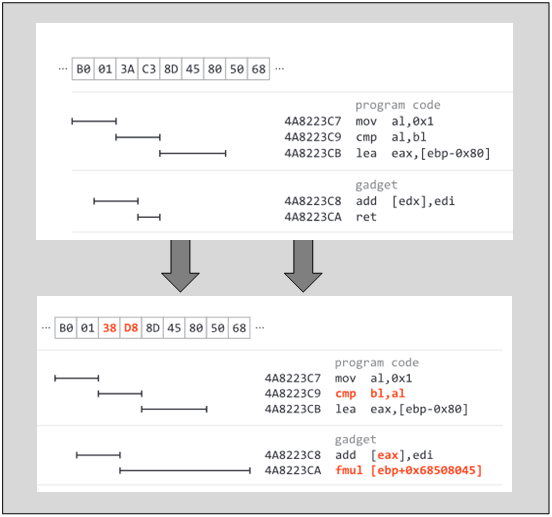
\includegraphics[width=0.75\textwidth]{figures/4.2}
	% \caption[这里的文字将会显示在 listoffigure 中]{这里的文字将会显示在正文中}
	\caption{Instruction Replacement Example }\label{fig:4.2}
\end{figure}

\item Reordering of Register Preservation Code:

This method is based on the theory that the sequence of push and pop instructions from callee-saved registers is alterable during function calls, which only need to follow the last-in-first-out (LIFO) stack rule. During function calls, the order of push (callee-saved registers) and corresponding pop instructions can vary if adhering to the last-in-first-out (LIFO) stack rule. Several push instructions are used by the function header to save data in registers, while corresponding pop instructions are used at the end of the function to restore values. Since the stack restores in reverse order, semantics during the entire process will be equivalent to the original if pop sequences are the opposite of push sequences.

\begin{figure}[hbt]
	\centering
	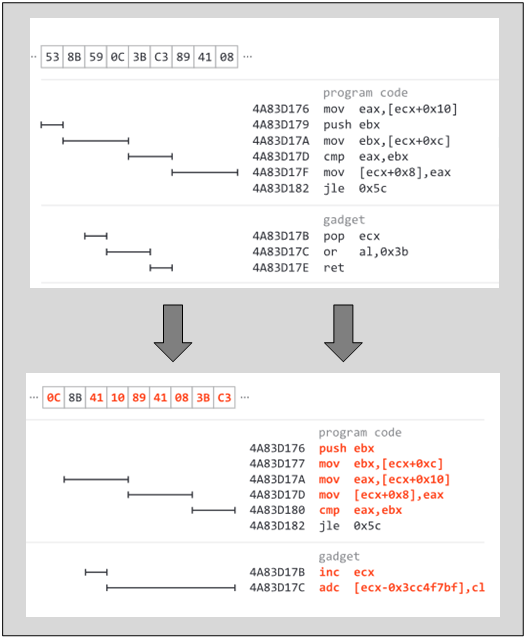
\includegraphics[width=0.75\textwidth]{figures/4.3}
	% \caption[这里的文字将会显示在 listoffigure 中]{这里的文字将会显示在正文中}
	\caption{Instruction Reordering Example}\label{fig:4.3}
\end{figure}

\begin{figure}[hbt]
	\centering
	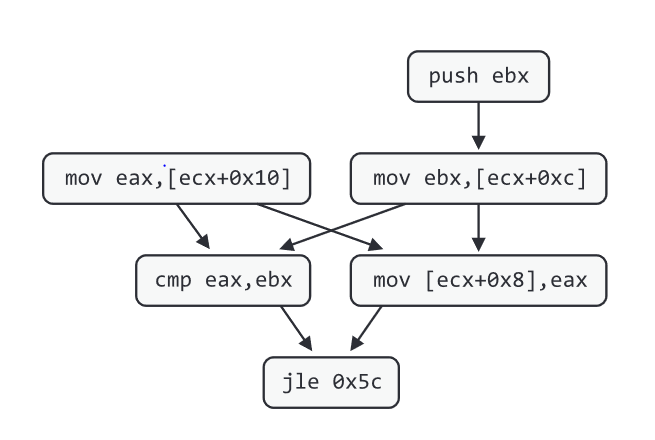
\includegraphics[width=0.75\textwidth]{figures/4.4}
	% \caption[这里的文字将会显示在 listoffigure 中]{这里的文字将会显示在正文中}
	\caption{Acyclic Graph of Reordered Instructions}\label{fig:4.4}
\end{figure}

\begin{figure}[hbt]
	\centering
	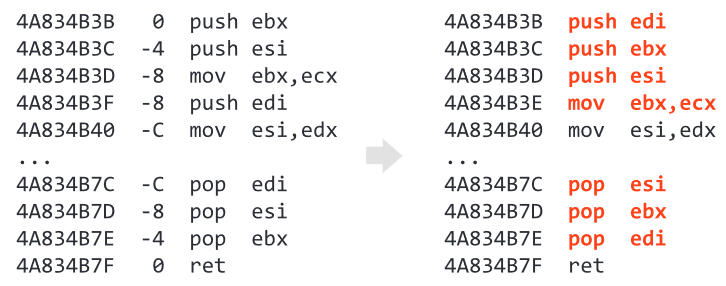
\includegraphics[width=0.75\textwidth]{figures/4.5}
	% \caption[这里的文字将会显示在 listoffigure 中]{这里的文字将会显示在正文中}
	\caption{Register Preservation Code Reordering Example}\label{fig:4.5}
\end{figure}

First, this method constructs the CFG for the binary program and performs register liveness analysis on each basic block to determine each instruction's register use and def sets. Second, this method iteratively computes each instruction's active in and out sets to identify live ranges in each register. On the premise that there is no conflict, two register pairs with non-overlapping live ranges are randomly selected, and then their usage positions are swapped in assembly. During instruction modification, modifying via ModR/M bytes (and SIB bytes if necessary) achieve remapping, avoiding special registers like ESP, filtering instructions with implicit register usage. To ensure call consistency, calling convention information is combined to constrain certain registers.

This technique does not introduce any new instructions or change operand values, modifying only register encodings at the machine-code level. It disrupts static analysis tools based on register usage patterns or feature sequences recognition strategies, enhancing sample adversariality and diversity.
\end{enumerate}



\begin{figure}[hbt]
	\centering
	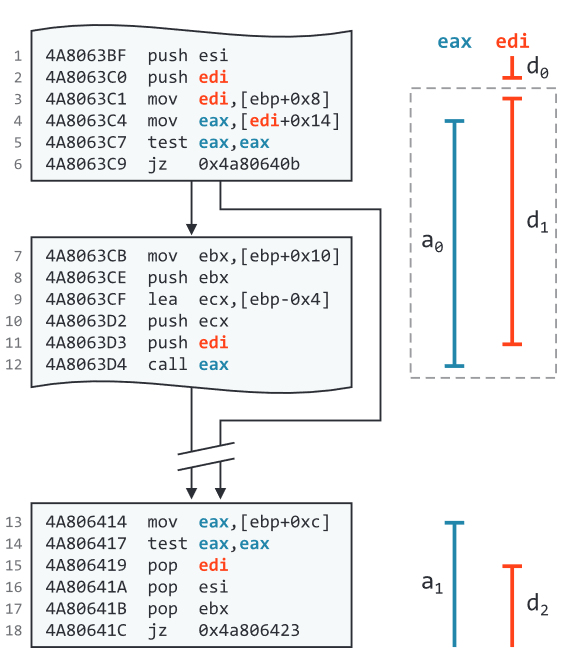
\includegraphics[width=0.75\textwidth]{figures/4.6}
	% \caption[这里的文字将会显示在 listoffigure 中]{这里的文字将会显示在正文中}
	\caption{Register Re-allocation Example}\label{fig:4.6}
\end{figure}

\subsection{Dynamic Behavior Disturbance Methods}

To balance efficiency and cost, dynamic analysis systems commonly allocate only a few seconds to dozens of seconds of execution time to each sample. For malware whose attack behaviors depend on conditional triggers or user interaction, this fixed analysis window presents a probability of being evaded.

Based on this observation, this research designs a dynamic disturbance method whose central mechanism is introducing "time-delay", deliberately waiting for a period after startup before executing core logic, making the malicious code evade the behavioral analysis window of sandboxes. This is primarily implemented by inserting delay logic like the nanosleep system call at program entry points or critical paths, ensuring that the malware exhibits no abnormal behavior during the initial run phase and thus bypasses detection systems based on behavioral features.

Specifically, this method inserts system call delay logic at the \_start entry point. It constructs a timespec structure to set the delay duration and invokes the nanosleep system call to induce suspension. During this delay, the sample remains dormant, triggering no system calls, memory reads and writes, network communications, or other suspicious activities. As most sandbox systems forcibly terminate processes after exceeding the execution time limit, the un-triggered malicious behavioral chain remains entirely unobserved. Consequently, even obviously destructive malware may be misclassified as benign due to "absence of malicious behavior."

\begin{algorithm}[htbp]
	\caption{使用可执行段填充空间进行 ELF 动态插入算法}
    \KwIn{目标 ELF 二进制文件路径 \texttt{input\_elf},载荷二进制代码路径 \texttt{code\_bin},输出 ELF 路径 \texttt{output\_elf}}
	\KwOut{一个已被感染的 ELF 文件,其中插入了载荷代码}
	Read the input ELF file \texttt{input\_elf} into memory \texttt{hdr}\;
	Read the payload binary code \texttt{code\_bin} into memory \texttt{code}\;
	Validate ELF magic number and ensure it is a 64-bit ELF\;
	Check if the ELF architecture is x86-64\;
	\ForEach{program header \texttt{phdr} in \texttt{hdr}}{
		\If{\texttt{phdr} is executable (has \texttt{PF\_X} flag)}{
			Find the last section \texttt{last\_sec} within \texttt{phdr}\;
			Compute the available padding size \texttt{pad\_size} after \texttt{last\_sec}\;
			\If{\texttt{pad\_size} $<$ size of \texttt{code} + size of jump}{
				Print error message and exit\;
			}
			Inject the payload \texttt{code} into the padding space\;
			Generate a jump instruction \texttt{jmp\_back} to the original entry point\;
			Inject \texttt{jmp\_back} after the \texttt{code}\;
			Modify the section header of \texttt{last\_sec} to extend its size\;
			Update the \texttt{phdr}'s file and memory size to include the injected code\;
			Update the ELF header's \texttt{e\_entry} to point to the start of the payload \texttt{code}\;
			\textbf{break}\;
		}
	}
	Write the modified ELF to \texttt{output\_elf}\;
	Set the file permission of \texttt{output\_elf} to executable\;
\end{algorithm}

The disturbance method based on time delay is an effective dynamic adversarial technique that has advantages in simple implementation, high efficiency, and high versatility. It serves as a key disturbance operation for malware in reinforcement learning training and adversarial generation. Its concrete implementation is described in Algorithm 1 below.

Algorithm 1 operates step-by-step, achieving inserting payload binary code into target ELF executable file's executable segment padding, maintaining original file structure while achieving control flow redirection. Lines 1 to 2 read target ELF file and payload into memory. Lines 3 to 4 check the legitimacy of ELF file, including magic number, whether it is 64 bits, and whether its architecture is x86-64. Lines 5 to 17 is the core process of injection, traversing each program header. Line 6 judges whether the segment is an executable segment that contains the PF\_X flag. Lines 7 to 8 locate the last section of this segment and calculate the gap size after it. Lines 9 to 10 terminate the process when the gap size cannot accommodate the payload and jump instructions. Lines 11 to 13 write the payload to the gap and append code block that jumps to the original entry point. Subsequently, lines 14 to 15 expand the size fields of the section and segment to cover newly injected areas to ensure that it can be loaded correctly during execution. Line 16 updates the entry point e\_entry in the ELF header to be the starting point of payload, achieving control flow redirection. Line 17 exits the loop to prevent duplicate operations after the injection is completed. Finally, lines 18 to 19 write the modified ELF file to an output file and set it as an executable file. The overall process achieves dynamic insertion operations that exhibit high concealment and complete compatibility in the condition that the original functionality is not broken.

\section{Reward Function Strategy Optimization}

In this research, designing the reward function for the RL model is a core element for generating adversarial malware samples. To enable the agent to effectively evade malware detection systems and generate adversarial samples with sufficient complexity, this research proposes a reward function that comprehensively considers evasion success, sample diversity, and generation complexity. The optimization and construction of the reward function directly determine the agent's learning effectiveness during training and final generated malicious samples' quality.

First, the primary goal of the reward function is to encourage the agent to generate malicious samples that can evade existing detection systems. Therefore, the reward function grants rewards based on whether the sample successfully evades detection. When the sample generated by the agent is not classified as malicious by the malware detection model, the agent receives a positive reward; otherwise, it receives a negative reward. This feedback mechanism guides the agent to continuously optimize its strategy during generation, thereby improving the evasion capability of malicious samples.

Second, sample diversity is also a critical factor that should be considered in the reward function. During adversarial sample generation process, if the agent increases sample diversity by modifying control flow, altering function call sequences, or inserting random strings, it receives corresponding rewards. This approach promotes the diversification of malicious samples, avoids generating monotonous or duplicate samples, and enhances the generalization ability of generated samples.

Finally, to prevent the agent from generating overly complex or unstable results, the reward function incorporates a penalty mechanism for sample complexity. If a generated malicious sample is excessively complex, such as containing too many control flow operations or lengthy code fragments, the agent is penalized. This strategy helps the agent generate more stable and effective samples while ensuring evasion capability and enhancing the practical application value of generated samples.

Traditional adversarial sample generation methods mostly adopt fixed or static reward functions, often considering only a single evasion detection result, such as whether the sample successfully evades a classifier or a sandbox analysis system\cite{anderson2018learning}. However, in real application scenarios, factors such as malware behavioral characteristics, detection mechanisms, and resource constraints, such as sandbox analysis duration, exhibit high dynamism. Therefore, this research designs an adaptive, stage-aware, and behaviorally sensitive dynamic reward function strategy that is significant for improving the quality and robustness of adversarial sample generation.

\subsection{Motivation for Reward Function Design}

The behavioral policy of a reinforcement learning agent is directly driven by its reward signals. If rewards are solely based on the singular signal of "whether evasion is successful," the agent may face sparse reward dilemmas during initial training phases, resulting in inefficient training, unstable strategies, or even failure to converge. To address this issue, this research proposes a method that introduces a multi-source reward signal fusion mechanism, integrating the following three metrics:
\begin{enumerate}
\item Evasion Score: It reflects whether the sample successfully evades sandbox or machine learning detection models, serving as the primary reward source.

\item Perturbation Cost: It measures the perturbation degree of modifications to the original sample, suppressing excessive alterations to maintain executability and semantic consistency.

\item Behavior Confusion Degree: It measures the similarity between sample behavior and benign software, encouraging the agent to generate more stealthy disturbance strategies.
\end{enumerate}

\subsection{Reward Function Formulation}
 
The reward $R_t$ for the agent after executing disturbance action $a_t$ at time $t$ is defined as a weighted combination:
\begin{equation}
	R_t = \lambda_1 \cdot R_{\text{evasion}} + \lambda_2 \cdot R_{\text{confusion}} - \lambda_3 \cdot R_{\text{cost}}
\end{equation}

In this formulation, $R_{\text{evasion}}$ represents that if the sample evade the sandbox or classifier, positive reward should be given, otherwise, the reward is zero; $R_{\text{confusion}}$ represents a score calculated from the similarity between behavioral sequence, such as system call graphs, and benign samples, such as using Jaccard similarity or structural similarity; $R_{\text{cost}}$ denotes the disturbance cost that is calculated based on number of disturbances, modified bytes, and sensitivity of modified locations; $\lambda_1$, $\lambda_2$, and $\lambda_3$ are dynamically adjustable weighting parameters.
\section{Reinforcement Learning Model Construction and Training}

The reinforcement learning model combining PPO and LSTM, proposed in this chapter, consists of four main components: an LSTM temporal feature encoding layer, a policy network (Actor), a value network (Critic), and a PPO optimizer. During the training process, first, the policy network generates an action probability distribution based on the current environment state. Concurrently, the value network evaluates the value of the current state. To effectively model temporal dependencies in action sequences, the LSTM module is introduced, which enables the model to record historical state information and capture long-term dependency features, enhancing policy stability and robustness. Finally, the PPO optimizer iteratively updates the policy, ensuring stable and efficient policy updates throughout the training process.

\begin{algorithm}[htbp]
	\caption{基于强化学习的 ELF 对抗样本生成算法}
	\KwIn{原始 ELF 恶意样本集 $S$,最大迭代次数 $I$,预训练模型 $M$(PPO+LSTM),免杀行为表 \texttt{Action\_table},检测结果记录表 \texttt{Re}}
	\KwOut{免杀后的样本集 $S$}
	初始化智能体 agent 与环境 env\;
	agent $\leftarrow$ PPO\_LSTM.load($M$)\;
	$R_d \leftarrow 0$\;
	\ForEach{$s \in S$}{
		env.reset()\;
		tag $\leftarrow$ env.detect($s$)\;
		$S_t \leftarrow [\ ]$\;
		\For{$i \leftarrow 1$ \KwTo $9$}{
			$S_t \leftarrow S_t + \texttt{env.extractor}(s, i)$\;
		}
		\For{$j \leftarrow 1$ \KwTo $I$}{
			act $\leftarrow$ agent.predict($S_t$, $R_d$)\;
			\If{tag == benign}{
				\textbf{break}\;
			}
			$s \leftarrow \texttt{env.step}(s, \texttt{Action\_table}[act])$\;
			$S_t \leftarrow [\ ]$\;
			\For{$i \leftarrow 1$ \KwTo $9$}{
				$S_t \leftarrow S_t + \texttt{env.extractor}(s, i)$\;
			}
			tag $\leftarrow$ env.detect($s$)\;
			
			计算规避性得分:\texttt{Evasion\_Score} $\leftarrow$ score\_function($s$)\;
			
			计算行为混淆度:\texttt{Behavior\_Confusion\_Degree} $\leftarrow$ calculate\_confusion\_degree($s$)\;
			
			计算扰动成本:\texttt{Perturbation\_Cost} $\leftarrow$ calculate\_perturbation\_cost($s$, \texttt{Action\_table}[act])\;
			
			\If{tag == benign}{
				$R_d \leftarrow 10 \cdot \texttt{coefficient1} + \texttt{Behavior\_Confusion\_Degree} - \texttt{Perturbation\_Cost}$\;
				\textbf{break}\;
			}
			\Else{
				$R_d \leftarrow \texttt{Behavior\_Confusion\_Degree} - \texttt{Perturbation\_Cost}$\;
			}
		}
		\texttt{Re[$s$]} $\leftarrow$ tag\;
	}
\end{algorithm}

Algorithm 2 describes the ELF-format malware adversarial sample generation process that uses a reinforcement learning model based on PPO and LSTM. Lines 1 to 2 initialize the agent and environment, loading the pre-trained PPO+LSTM model. Line 3 initializes the reward signal $R_d$ to 0. Lines 4 to 6 iterate through the original malicious sample set $S$, reset the environment, and detect the sample's label. Lines 7 to 9 extract features from the environment and store them in state $S_t$. Lines 10 to 26 are the core disturbance steps: the agent predicts an action based on the current state and reward signal. Lines 11 to 12 generate disturbance actions based on the agent's prediction and decide whether to continue according to whether the sample's label is benign or malicious. After executing actions, lines 13 to 15 update samples and extract novel environmental characteristics. Line 16 to 18 calculate novel reward value comprehensively based on evasion score, behavior confusion degree, and disturbance cost. Line 19 to 24 dynamically calculates reward values according to the detection result and disturbance cost. If the sample evades detection successfully, higher rewards will be granted. Otherwise, the disturbance cost is calculated, and rewards are penalized. Line 27 updates the sample's label and records it in the result table Re. The whole process gradually optimizes the agent's strategies through merging multi-source signals and adjusting dynamically, generating adversarial samples that evade detection effectively while maintaining executability.

\subsection{LSTM Temporal Feature Encoding Layer}

In traditional RL, policy and value estimation usually rely solely on single-step decisions based on the current state, neglecting temporal correlations among historical decisions. This can lead to short-sighted behavior.

To address this issue, the model introduces an LSTM layer at the input stage. Through gating mechanisms, LSTM captures long-term dependencies, enhancing the temporal coherence of decision-making.

Internal operation formulations of the LSTM unit are defined as follows:

Input Gate (controlling the flow of current input information):
\begin{equation}
i_t = \sigma(W_i x_t + U_i h_{t-1} + b_i)
\end{equation}

Forget Gate (controlling retention level of the previous memory cell):
\begin{equation}
f_t = \sigma(W_f x_t + U_f h_{t-1} + b_f)
\end{equation}

Cell State Update (Generating new memory content):
\begin{equation}
\tilde{c}_t = \tanh(W_c x_t + U_c h_{t-1} + b_c)
\end{equation}

Cell State Update (memory cell):
\begin{equation}
c_t = f_t \odot c_{t-1} + i_t \odot \tilde{c}_t
\end{equation}

Output Gate (controlling hidden state output):
\begin{equation}
o_t = \sigma(W_o x_t + U_o h_{t-1} + b_o)
\end{equation}

Hidden State Update (output for the next step):
\begin{equation}
h_t = o_t \odot \tanh(c_t)
\end{equation}

In the formulations, $\sigma$ is the Sigmoid activation function. $\odot$ represents the Hadamard product in element multiplication. $x_t$ is the input state of current time. $h_{t-1}$ and $c_{t-1}$ are the hidden state and cell state of the previous time step.

This mechanism enables the LSTM to effectively capture long-term dependencies in input state sequences, enhancing the historical modeling capability of the policy and value networks.

\subsection{Policy Network (Actor)}

The policy network receives environmental state information and outputs the probability distribution of current actions. To enhance its awareness of historical information, the policy network introduces an LSTM layer at the input stage. The LSTM records hidden information from previous states, enabling the output policy to rely on not only the current observation but also features from historical observation sequences. The policy network's goal is to output each action's probability distribution $\pi_{\theta}(a_{t}|s_{t})$ based on the current hidden state $h_{t}$. The concrete processes are listed below:

\begin{enumerate} [label=\arabic*)] 

\item The LSTM-encoded hidden state $h_{t}$ serves as input.

\item A multilayer perceptron (MLP) maps this to the action space.

\item The Softmax function outputs the action distribution:
\begin{equation}
\pi_{\theta}(a_t | s_t) = Softmax(W_p h_t + b_p)
\tag{4.8}
\end{equation}
In this formulation, $W_p$ and $b_p$ are the policy network's weight and bias parameters, and $\theta$ represents the policy network's parameter set.

\item Actions $a_t$ are generated according to the sampling from the probability distribution.
\begin{equation}
a_t \sim \pi_\theta(a_t | s_t)
\end{equation}

\end{enumerate}

\subsection{Value Network (Critic)}

The value network estimates the value of the current state and predicts the expected cumulative reward obtained by following the current policy starting from the current state. Like the policy network, the value network introduces an LSTM encoding layer to capture temporal correlations in state sequences, enhancing estimation accuracy and stability.

The value network aims to estimate the state-value function $V^{\pi}(s_{t})$ in current state $s_{t}$, the expected total reward from state $s_t$ following current strategy $\pi$. Like the structure of strategy networks, value networks are also based on the LSTM-encoded hidden state $h_{t}$ and output a scalar value through MLP.

State value estimation:
\begin{equation}
V_{\phi}(s_t) = W_v h_t + b_v
\end{equation}

In this formulation, $W_v$ and $b_v$ are the weight and bias parameters of the value network, and $\phi$ denotes its parameter set.

\subsection{Policy Optimizer}

PPO introduces a clipped objective function that limits the divergence between old and new policies during updates, enhancing training stability.

First,the probability ratio $r_t(\theta)$ is defined as:
\begin{equation}
	r_t(\theta) = \frac{\pi_{\theta}(a_t | s_t)}{\pi_{\theta_{\text{old}}}(a_t | s_t)} \tag{4.11}
\end{equation}

$\pi_{\theta_{\text{old}}}$ represents the pre-update policy parameters.

The advantage function $A_t$ is defined as:
\begin{equation}
	A_t = \delta_t = r_t + \gamma V(s_{t+1}) - V(s_t) \tag{4.12}
\end{equation}

$r_t$ is the immediate reward and $\gamma$ is the discount factor.

PPO's ultimate optimization target is:
\begin{equation}
	L^{\text{CLIP}}(\theta) = \mathbb{E}_t \left[ \min \left( r_t(\theta) A_t, \ \text{clip}\big(r_t(\theta), 1-\epsilon, 1+\epsilon\big) A_t \right) \right] \tag{4.13}
\end{equation}

When \(r_t(\theta)\) lies in the range \((1-\epsilon, 1+\epsilon)\), the true ratio multiplied by the advantage function is used. Outside this range, the clipped ratio is used to prevent excessive policy updates.

The value function loss (squared error) is:
\begin{equation}
	L^{\text{VF}}(\varphi) = \mathbb{E}_t \left[ \left(V_{\varphi}(s_t) - R_t\right)^2 \right] \tag{4.14}
\end{equation}

In this formulation, $R_t$ is the cumulative return (real value target).

The ultimate overall loss function combining policy loss, value loss, and entropy regularization is:
\begin{equation}
	L(\theta, \varphi) = L^{\text{CLIP}}(\theta) - c_1 L^{\text{VF}}(\varphi) + c_2 S[\pi_{\theta}] \tag{4.15}
\end{equation}

Where \(S[\pi_{\theta}]\) is the policy entropy to encourage exploration. \(c_1\) and \(c_2\) are weighting coefficients.

